\title{Article Title}

\author{William Cutler, Jack Donaghue, Haridas Kumarakuru, Don Heiman}

\newcommand{\abstractText}{\noindent
The unique optical properties of the ruby crystal that make it particularly effective as a lasing medium were measured using an inexpensive setup. Ruby’s absorption of visible light was shown to be strongest at \SI{420}{\nm} and \SI{550}{\nm}, corresponding to its physical appearance as translucent and pink. While the ruby crystal was illuminated with a \SI{532}{\nm} green laser, the R-line fluorescence peaked at \SI{693.8\pm1.1}{\nm}. Finally, the fluorescence lifetime of ruby was measured by pulsing the laser with a signal generator and capturing the decaying light waveform on a digital oscilloscope via a high-speed photodiode. An exponential decay time-constant of \SI{3.6\pm0.1}{\ms} was obtained and will be discussed further in this paper. 
}

%%%%%%%%%%%%%%%%%
% Configuration %
%%%%%%%%%%%%%%%%%

\documentclass[11pt, a4paper, twocolumn]{article}
\usepackage{xurl}
\usepackage[comma,sort&compress]{natbib}
\usepackage{abstract}
\usepackage[separate-uncertainty=true]{siunitx}
\usepackage{graphicx}
\renewcommand{\abstractnamefont}{\normalfont\bfseries}
\renewcommand{\abstracttextfont}{\normalfont\small\itshape}
\usepackage{lipsum}

% Any configuration that should be done before the end of the preamble:
\usepackage{hyperref}
\usepackage{float}
\hypersetup{colorlinks=true, urlcolor=blue, linkcolor=blue, citecolor=blue}
\usepackage[a4paper, total={7in, 10in}]{geometry}
\setlength{\columnsep}{24pt}
\begin{document}

%%%%%%%%%%%%
% Abstract %
%%%%%%%%%%%%

\twocolumn[
  \begin{@twocolumnfalse}
    \maketitle
    \begin{abstract}
      \abstractText
      \newline
      \newline
    \end{abstract}
  \end{@twocolumnfalse}
]

%%%%%%%%%%%
% Article %
%%%%%%%%%%%

\section*{Introduction}
The absorption and fluorescence emission spectra have long been used to identify, characterize, and study materials \cite{BrittanicaSpectroscopy}. In lasing mediums such as ruby, these properties govern its excitation and emission spectra respectively. Studies of ruby absorption typically use a spectrophotometer and measure two broad absorption peaks centered near \SI{410}{\nm} and \SI{550}{\nm} \cite{Esposti,Kusuma,Song}. Devices with high resolution (\SI{0.5}{\nm} slit width) additionally detect a small doublet absorption peak near \SI{694}{\nm}. Song et. al. find absorption peaks at \SI{410}{\nm} and \SI{550}{\nm}, and calculates an absorption coefficient from these values according to Beer-Lambert's law.

The room temperature fluorescence spectrum of ruby has been reported well throughout the early 1900's with a double peak at \SI{692.7}{\nm} and \SI{694.2}{\nm}, corresponding to the characteristic $R_1$ and $R_2$ lines \cite{Kumari, Mani}. With lower resolution instruments, only a single primary peak was detected at \SI{694.2}{\nm} by Esposti et. al. Other fluorescence lines have been detected near these peaks at 671, 688, 695, and \SI{710}{\nm} \cite{Kusuma}.

The effectiveness of ruby as a lasing medium depends on its ability to maintain a population inversion between the ground state and the meta-stable state. The stability of this meta-stable state can be measured by the fluorescence lifetime, which relates to how long the crystal will fluoresce in the absence of pumping, and therefore the time for which there is a size-able meta-stable population. Whereas most materials have nano or picosecond fluorescence lifetimes \cite{Berezin}, ruby’s fluorescence lasts milliseconds, and long enough to hold a population inversion for a working laser.

\begin{figure}
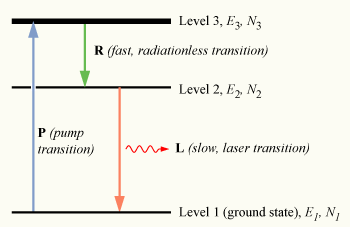
\includegraphics[width=\linewidth]{Population-inversion-3level.png}
\caption{Sample energy level diagram showing three phases of fluorescence: pumping, non-radiative relaxation, and fluorescent relaxation}
\label{fig:populationInversion}
\end{figure}

The fluorescence lifetime of around \SI{3.5}{\ms} is typically reported, but this measurement is dependent on a number of factors. Investigations of the temperature dependence show that lifetime decreases for temperatures above room temperature \cite{Seat, Nelson}. Investigations of the dependence on ruby diameter show an increasing fluorescence lifetime with increased size as emitted photons are reabsorbed more frequently in larger samples \cite{Jones}. The effect of doping concentration changes dramatically with the temperature as found by \cite{Brown}. Brown found that at room temperature, doping concentrations between 0.005\% and 0.1\% yielded lifetimes in the range of 3-\SI{4}{\ms}.

Many investigations use a single-exponential fit to obtain the fluorescence lifetime, but others use a double-exponential fit based on the shape of their residuals \cite{McBane, Jones}. There is also some variation on whether a background constant is accounted for, but without it, we found a lifetime further from the typical \SI{3.5}{\ms} and closer to the \SI{4.2}{\ms} reported by Esposti.
\section*{Results}
\subsection*{Absorption and Transmission}

\begin{figure}[H]
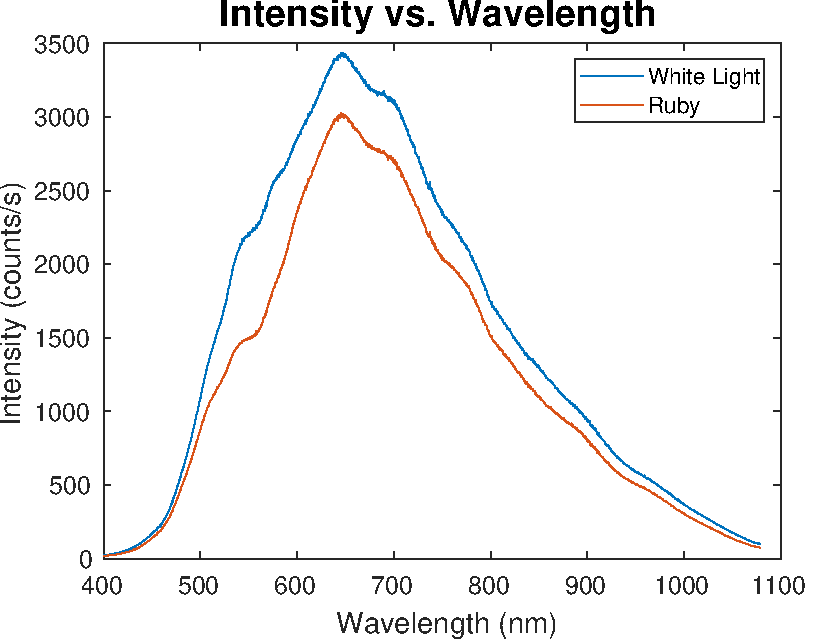
\includegraphics[width=\linewidth]{doubleIntensityMeasurement.pdf}
\caption{Spectrum of intensities for bare white light and white light passing through ruby
}
\label{fig:intensities}
\end{figure}

\begin{figure}[H]
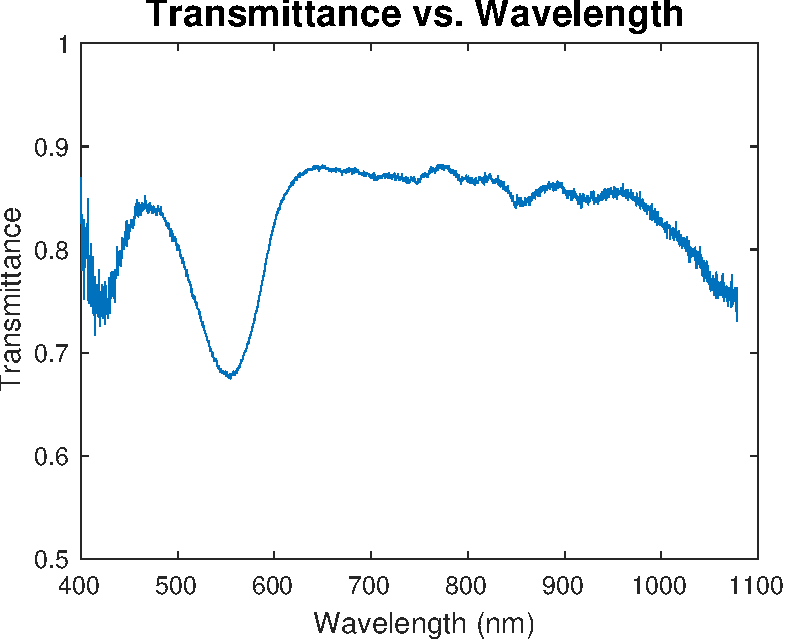
\includegraphics[width=\linewidth]{transmissionSpectrum.pdf}
\caption{Transmission spectrum of the ruby crystal showing prominent valleys at 420 nm and 550 nm}
\label{fig:intensities}
\end{figure}

\begin{figure}[H]
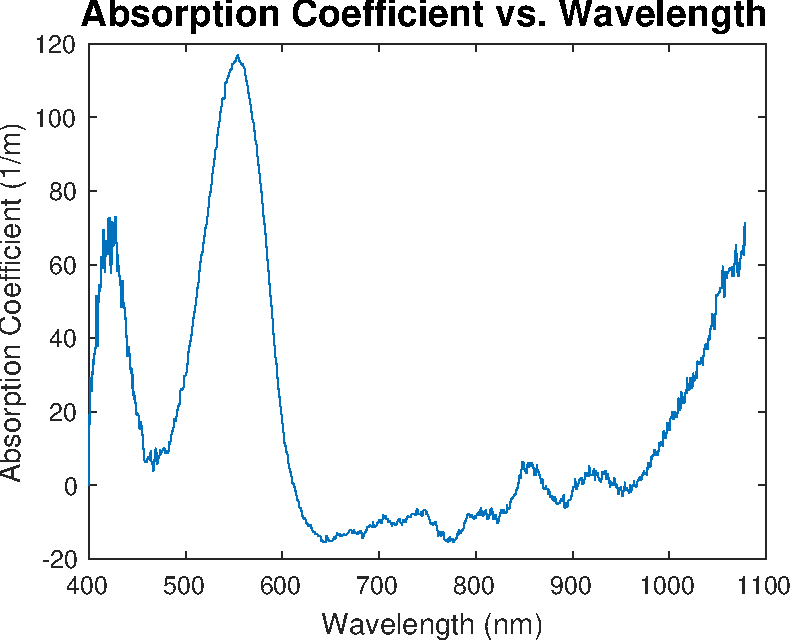
\includegraphics[width=\linewidth]{absorptionSpectrum.pdf}
\caption{Absorption spectrum of the ruby crystal with two absorption peaks centered at 410 nm and 550 nm}
\label{fig:intensities}
\end{figure}

\begin{figure}[H]
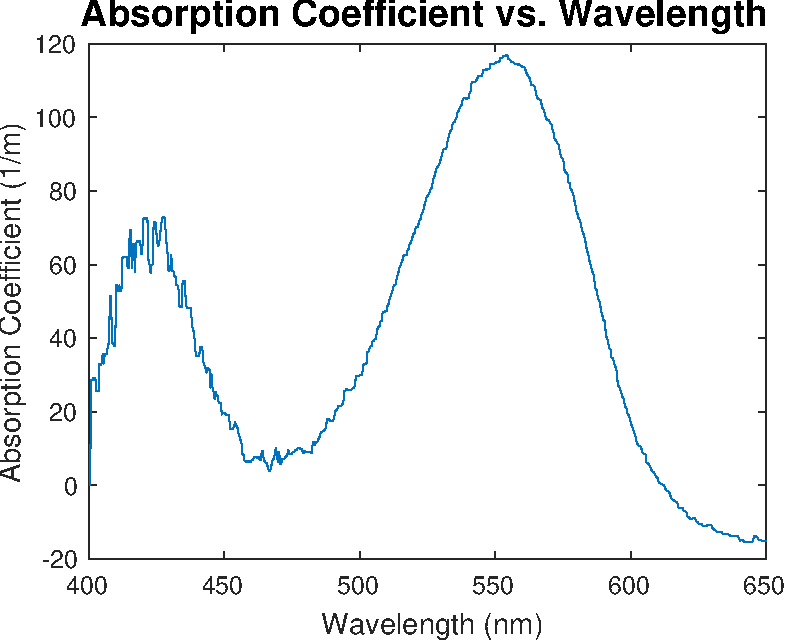
\includegraphics[width=\linewidth]{absorptionSpectrumFocused.pdf}
\caption{Focused absorption spectrum on the visible light wavelengths}
\label{fig:intensities}
\end{figure}

\begin{figure}[H]
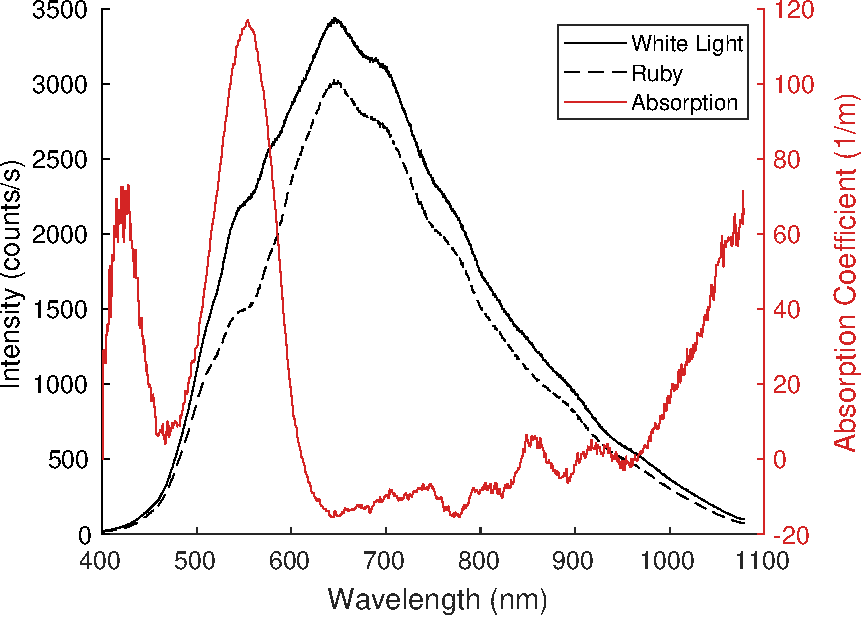
\includegraphics[width=\linewidth]{absorptionAndIntensitySpectra.pdf}
\caption{ Combination of intensity and absorption spectra showing a correspondence between the strongest absorption peak and intensity differential between measurements with and without ruby
}
\label{fig:intensities}
\end{figure}

\begin{figure}[H]
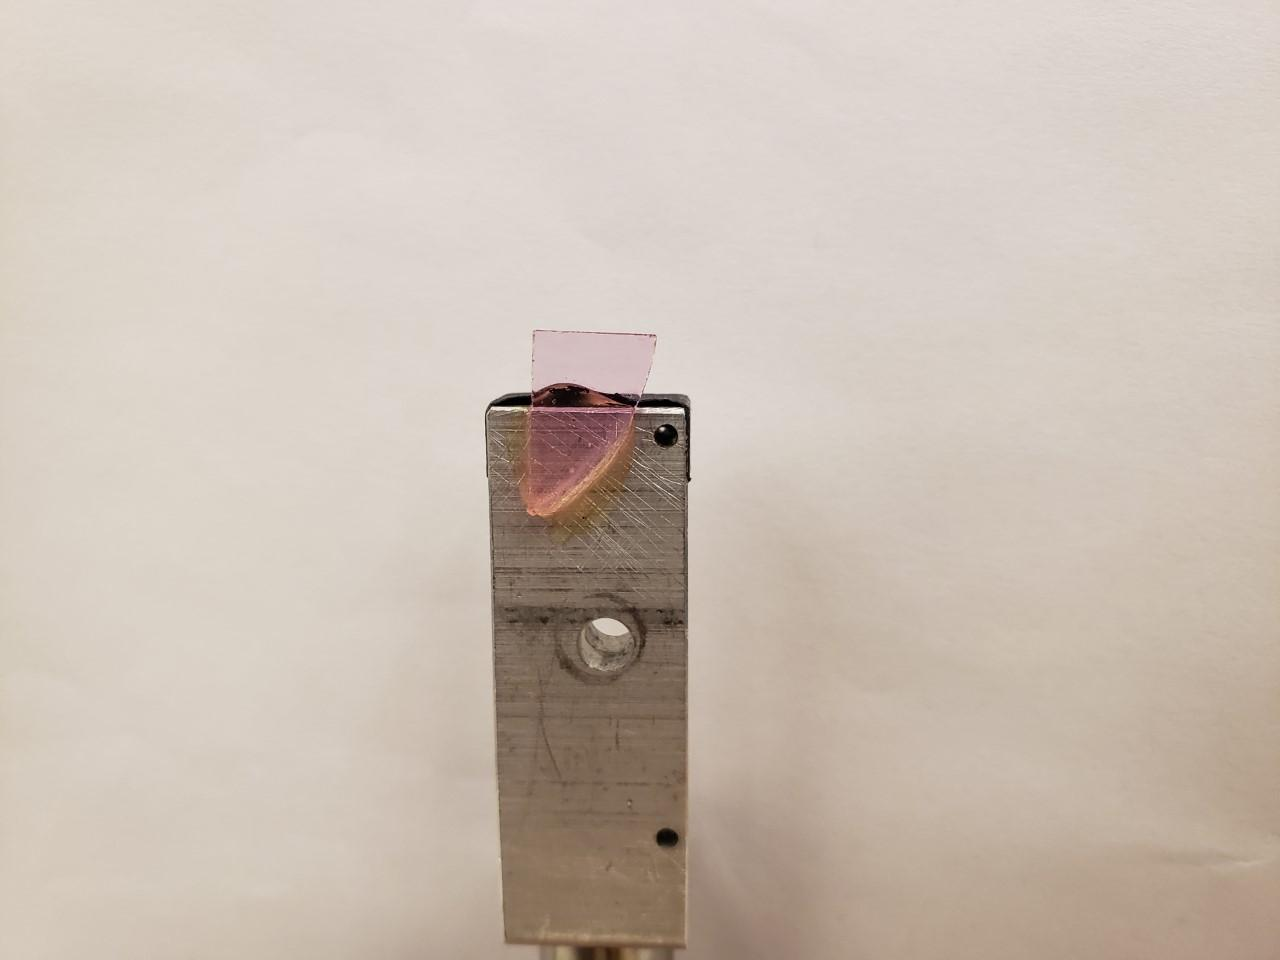
\includegraphics[width=\linewidth]{rubyPhoto.png}
\caption{Photograph of the transparent pink ruby crystal used throughout this study. Lasers and lights were directed to the top part of the crystal, above the metal stand
}
\label{fig:intensities}
\end{figure}

\subsection*{Fluorescence Spectrum}
R-line fluorescence was initiated in ruby by directing a constant \SI{532}{\nm} green diode laser beam into the crystal. The resulting fluorescent light was captured by a collection lens and directed through a fiber optic cable to the spectrometer for measurement. A black cloth covered the breadboard to eliminate background light.

A white light was shined through the fiber optic to aid in focusing the fluorescence on the fiber optic cable. Additionally, the laser was briefly fired during this adjustment to ensure that the focused white light and laser both struck the ruby at the same location.
Peak R-Line fluorescence occurred at \SI{693.5\pm1.1}{\nm}, a deep red color. Although in the visible spectrum, the red fluorescent light itself was not visible due to its low intensity, and could only be detected by the spectrograph. The peak observed actually corresponds to a doublet peak at 692.7 and \SI{694.3}{\nm} measured in more precise experiments -  the spectrograph used has limited resolution, resulting in one large peak in between this doublet. Also captured by the spectrograph are smaller peaks on either side of the primary R-line, at \SI{670}{\nm} and \SI{710}{\nm}, corresponding to Neighbor (N) lines and side bands respectively.

\begin{figure}[H]
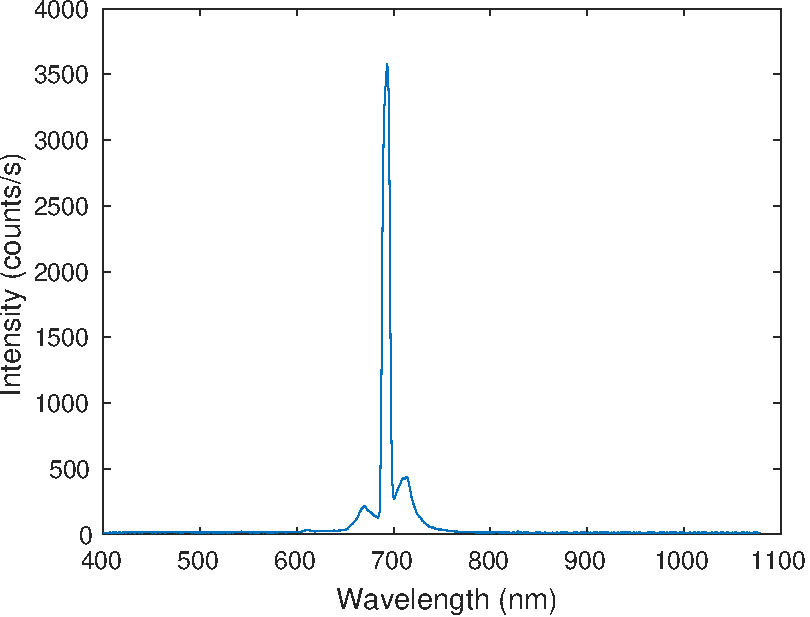
\includegraphics[width=\linewidth]{fluorescenceSpectrum.pdf}
\caption{Fluorescence spectrum resulting from 532 nm excitation laser showing R-line fluorescence at 693.5 nm}
\label{fig:intensities}
\end{figure}

\begin{figure}[H]
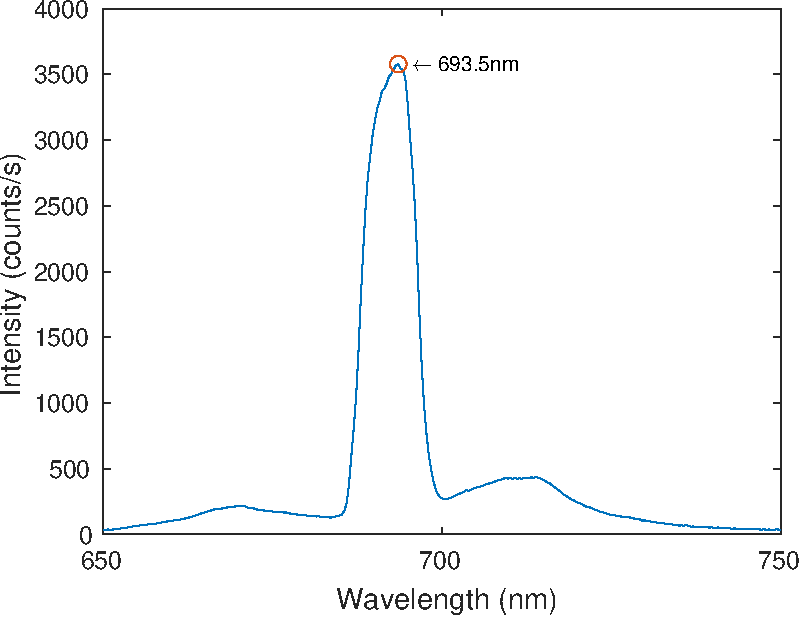
\includegraphics[width=\linewidth]{fluorescenceSpectrumFocused.pdf}
\caption{Focused fluorescence spectrum showing fluorescence peak}
\label{fig:intensities}
\end{figure}

\begin{figure}[H]
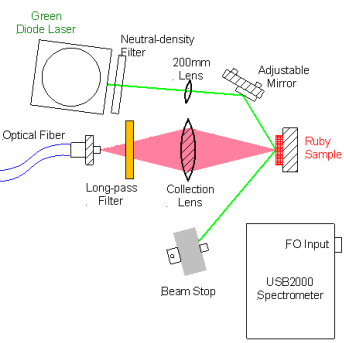
\includegraphics[width=\linewidth]{laserBenchDiagram.png}
\caption{Diagram of fluorescence spectrum measurement setup showing the laser beam in green and R-line fluorescence in red
}
\label{fig:intensities}
\end{figure}

The “efficiency” of the emitted light can be approximated from the ratio of the input wavelength to the output, yielding 532/693.5 = 76.7\%. That is, an R-line fluorescence photon has 76.7\% the energy of the green laser photon absorbed from the relation $E = hc/\lambda$. This is consistent with the non-radiative relaxation step of fluorescence that necessitates that the meta-stable state is of lower energy than the initial excited state.

\subsection*{Fluorescence Lifetime}

\begin{figure}[H]
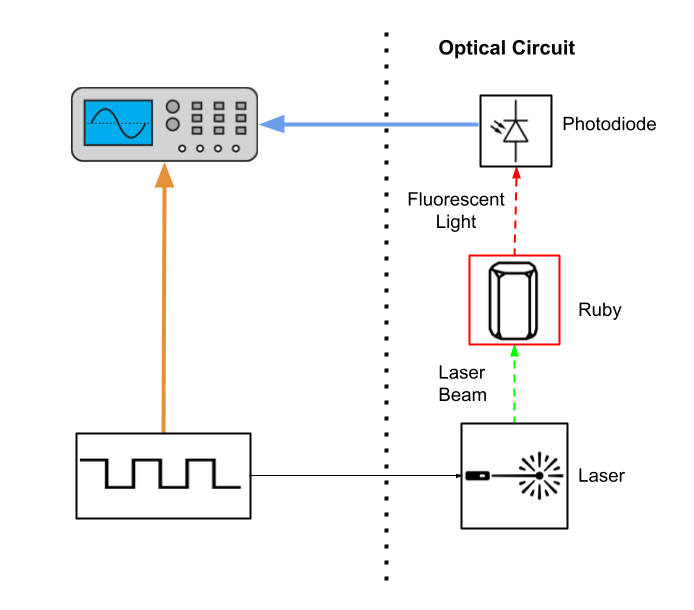
\includegraphics[width=\linewidth]{decayMeasurementSchematic.png}
\caption{Abstract schematic of fluorescence lifetime measurement showing how the square-wave and the signal path via laser and fluorescence reach the oscilloscope}
\label{fig:intensities}
\end{figure}

\begin{figure}[H]
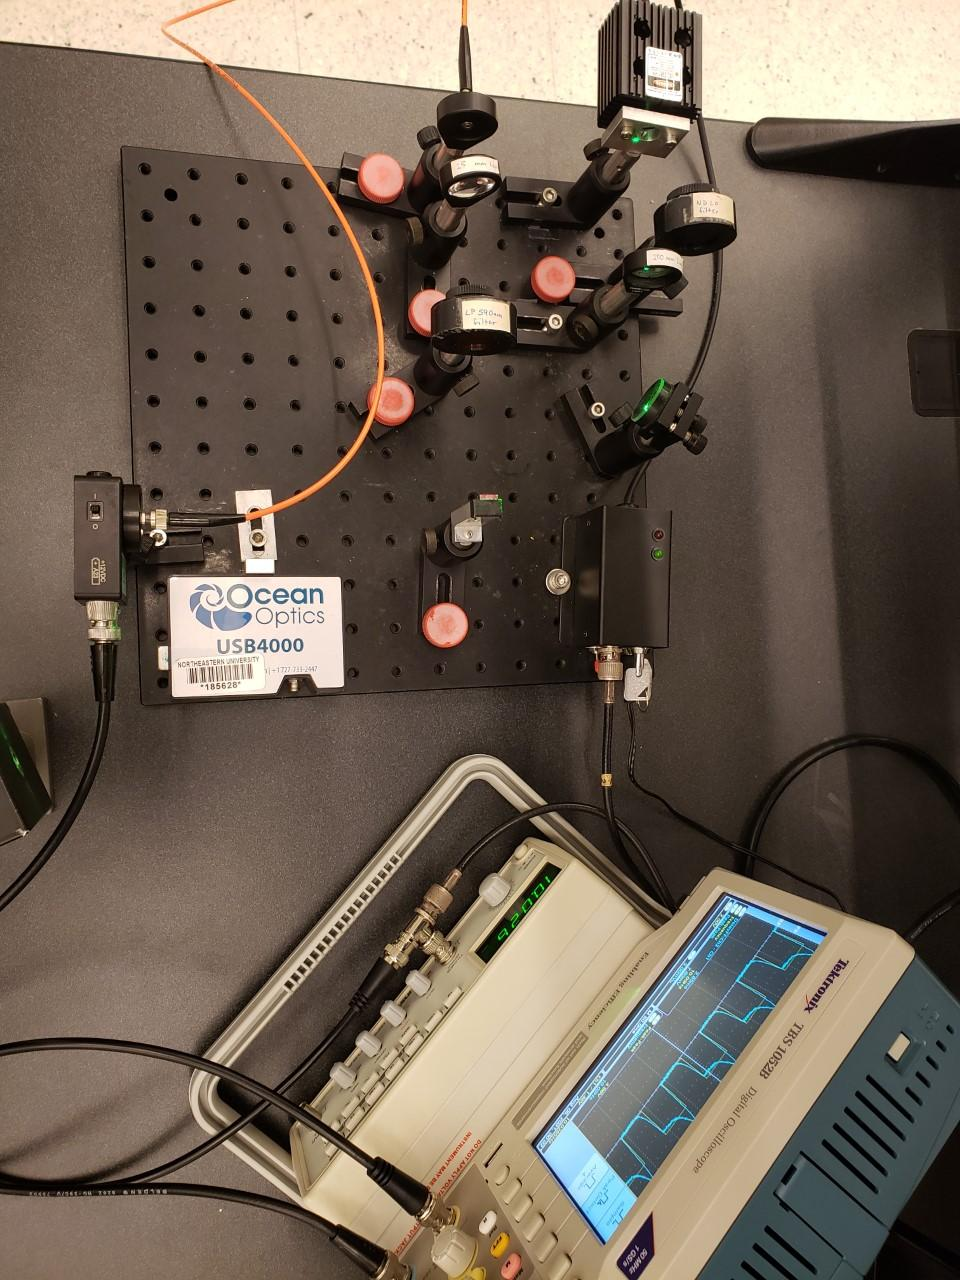
\includegraphics[width=\linewidth, height=\linewidth]{laserBenchPhoto.png}
\caption{Diagram of fluorescence spectrum measurement setup showing the laser beam in green and R-line fluorescence in red
}
\label{fig:intensities}
\end{figure}

Important aspects of the fluorescence process were observed by measuring the strength of fluorescence across time for a ruby crystal subjected to a pulsed laser. The diagram below shows an abstracted setup in which the laser is pulsed by a 10 Hz square wave function generator and the ruby fluorescence is captured by a photodiode. An oscilloscope simultaneously records the square wave that pulses the laser and the fluorescence signal captured by the photodiode.

\begin{figure}[H]
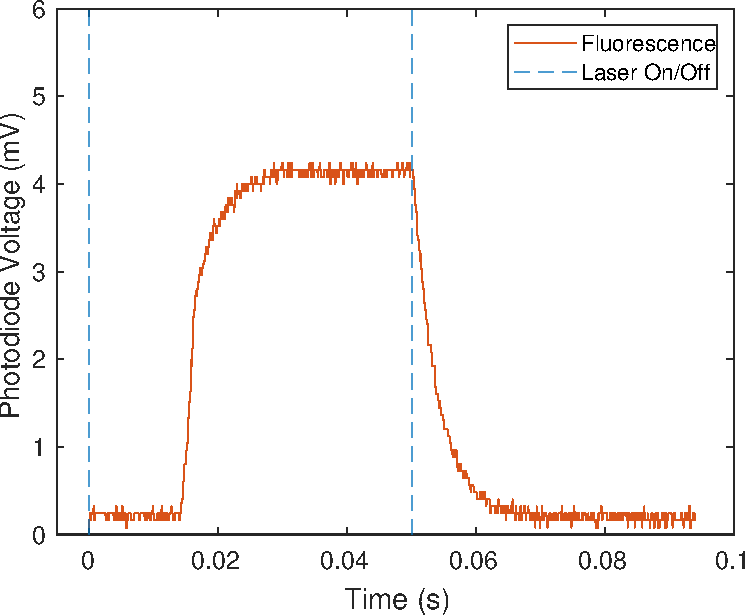
\includegraphics[width=\linewidth]{fluorescencePeriod.pdf}
\caption{Oscilloscope data for one period of laser pulse at 10 Hz showing the time-correspondence between the laser activation (blue) and measured fluorescence rate (orange}
\label{fig:intensities}
\end{figure}

\begin{figure}[H]
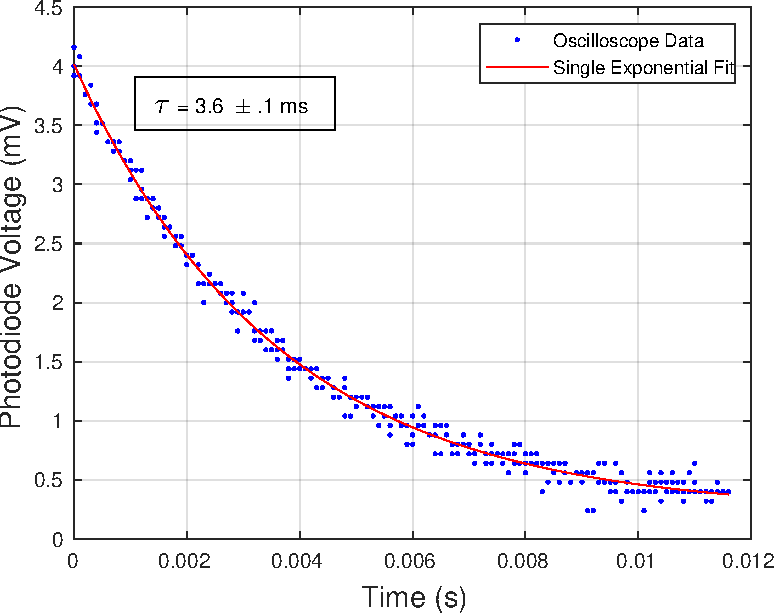
\includegraphics[width=\linewidth]{decayFit.pdf}
\caption{Exponential curve fit performed in MATLAB to determine the decay constant for fluorescence decay
}
\label{fig:populationInversion}
\end{figure}

\begin{figure}[H]
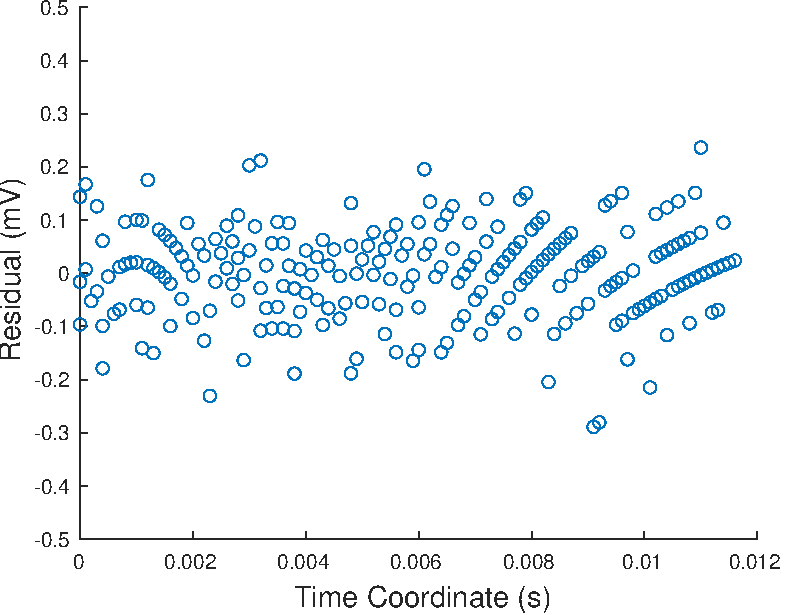
\includegraphics[width=\linewidth]{decayResiduals.pdf}
\caption{Residual plot for the single exponential fit showing no discernible pattern that might indicate a more complex fit is needed.}
\label{fig:intensities}
\end{figure}

The figure on the right shows one period of the 10 Hz signal recorded on the oscilloscope, with the square wave in blue and the fluorescence in orange. It shows a series of distinct phases outlining the entire process of fluorescence. No fluorescence occurs during the first 0.175 seconds after the laser is fired, indicating a period of laser absorption, chromium excitation, and non-radiative relaxation. The fluorescence rises sharply t = .015 to t = .025, as chromium ions relax back to the ground state. From t = .025 until the laser pulse turns off at t = .05, the rate of fluorescence is saturated, so it does not increase further. Finally, after t = .05, with the laser turned off, fluorescence continues, and the rate of fluorescence decreases exponentially. 
The rate of this exponential decay is governed by the probability that a given meta-stable chromium atom will fluoresce and relax in a given period of time. For the period of time chosen, the smaller this probability of decay, the more stable the meta-stable state is. Using this, the rate of exponential decay can be used to obtain a “decay time” that indicates how stable the R-Line meta-stable state is.

The fluorescence decay was isolated from the oscilloscope data, and a single exponential fit of the form $y = ae^{-x/\tau} + c$ was applied to determine the time constant for the decay, $\tau$, for which a value of \SI{3.6\pm0.1}{\ms} was obtained. The inclusion of a constant in the fit was important because the photodiode voltage does not decay to 0, but to some background value.

The time constant represents the amount of time for the fluorescence decay rate to decrease to 1/e of its original value, and is equivalent to the fluorescence lifetime. Whereas many materials exhibit fluorescence lifetimes on the order of ns or ps, ruby’s fluorescence lasts multiple milliseconds, and is a significant factor in its effectiveness as a lasing medium.

\section*{Discussion}
The tests performed concern the optical properties of the ruby crystal sample. The absorption spectrum was found to have peak absorptions at wavelengths of 420 ± 5 nm and 553 ± 1 nm with absorption depths of 15.0 ± 2.2 mm and 8.57 ± 0.08 mm respectively. The transmission and absorption spectra of the ruby were consistent with its visual appearance as a pink translucent crystal. The fluorescence showed a singular clear peak at 693.5 ± 1.1 nm. This range would encompass the double line of the ruby fluorescence spectrum at 692 and 694 nm recorded by (cite source). It also means that the fluorescence has 76.7\% of the energy from the 532nm laser used to excite the ruby. The R-Line fluorescence lifetime was found to be equal to 3.6 ± 0.1 ms.

The results of the experiment would be affected by light from the laboratory if the black cloth used to cover the optic setup were to allow a small amount of light to enter the setup and affect the ruby or spectrometer. Also any dust, oil, or other impurities touching the laser, ruby, spectrometer, or optical component would likewise have changed the measurements and introduced sources of error.

\subsection*{Acknowledgements}
We would like to thank Nathaniel Avish and Hongwei Chen, for their help in the laboratory and as teaching assistants for the Advanced Physics Laboratory section for which this experiment was introduced. We would also like to thank the Northeastern University Department of Physics for supporting our experience at the conference financially.
%%%%%%%%%%%%%%
% References %
%%%%%%%%%%%%%%

\nocite{*}
\bibliographystyle{plain}
\bibliography{reference}

\end{document}

